% !TEX root = ../main.tex
\appendix
\chapter{Appendix}

\section{HPLC Methods} % (fold)
\label{sec:hplc_methods}

	Vielleicht wenn hier text steht

	\begin{table}[htbp]
		\caption[Standard C18 screening method]{\textbf{Standard C18 screening method}}
		\label{tab:method_c18_screening}
		\centering
		\begin{tabularx}{\textwidth}{XX}
			\toprule
			\textbf{Parameter}	& \textbf{Value}	\\
			\midrule
			Column 		& Nucleosil-100 C18 \SI{5}{\micro\meter} 150$\times$\SI{3}{\milli\meter} 	\\
			Solvents	& A: Water + 0.1~\% Formic acid 	\\
						& B: Acetonitrile + 0.1~\% Formic acid		\\
			Method 		& Gradient 5 - 100 \% B for \SI{15}{\minute} 	\\
						& Plateau 100 \% B for \SI{3}{\minute} 	\\
			Flow 		& \SI{0.85}{\milli\liter\per\minute} \\
			Temperature & \SI{25}{\celsius} 	\\
			Injection Volume 	& \SI{50}{\micro\liter} 	\\
			\bottomrule
		\end{tabularx}
	\end{table}

	\begin{table}[htbp]
		\caption[Standard aminocolumn method]{\textbf{Standard aminocolumn method}}
		\label{tab:method_nh2_standard}
		\centering
		\begin{tabularx}{\textwidth}{XX}
			\toprule
			\textbf{Parameter}	& \textbf{Value}	\\
			\midrule
			Column 		& Luna NH2 \SI{5}{\micro\meter} 250$\times$\SI{4.6}{\milli\meter} 	\\
			Solvents	& A: Water + 0.1~\% Formic acid 	\\
						& B: Acetonitrile + 0.1~\% Formic acid		\\
			Method 		& Isocratic 80~\% B for \SI{20}{\minute} 	\\
						& + 100~\% A for \SI{10}{\minute}   \\
			Flow 		& \SI{2}{\milli\liter\per\minute} \\
			Temperature & \SI{25}{\celsius} 	\\
			Injection Volume 	& \SI{50}{\micro\liter} 	\\
			\bottomrule
		\end{tabularx}
	\end{table}

	\begin{table}[htbp]
		\caption[Aminocolumn method adapted for MS coupling]{\textbf{Aminocolumn method adapted for MS coupling}}
		\label{tab:method_nh2_ms}
		\centering
		\begin{tabularx}{\textwidth}{XX}
			\toprule
			\textbf{Parameter}	& \textbf{Value}	\\
			\midrule
			Column 		& Luna NH2 \SI{5}{\micro\meter} 250$\times$\SI{4.6}{\milli\meter} 	\\
			Solvents	& A: Water + 0.1~\% Formic acid 	\\
						& B: Acetonitrile + 0.1~\% Formic acid		\\
			Method 		& Isocratic 80~\% B for 60 min. 	\\
			Flow 		& \SI{0.5}{\milli\liter\per\minute} \\
			Temperature & \SI{40}{\celsius} 	\\
			Injection Volume 	& \SI{50}{\micro\liter} 	\\
			\midrule
			Capillary Voltage 		& \SI{3500}{\volt} 	\\
			Injector Temperature	& \SI{350}{\celsius}\\
			Target mass 			& 400 m/z 			\\
			\bottomrule
		\end{tabularx}
	\end{table}

	\begin{table}[htbp]
		\caption[The standard ZIC-HILIC method]{\textbf{The standard ZIC-HILIC method}}
		\label{tab:method_hilic_standard}
		\centering
		\begin{tabularx}{\textwidth}{XX}
			\toprule
			\textbf{Parameter}	& \textbf{Value}	\\
			\midrule
			Column 		& ZIC-HILIC \SI{3.5}{\micro\meter} 150$\times$\SI{4.6}{\milli\meter} 	\\
			Solvents	& A: 	10~mM Ammonium acetate 	\\
						& B: 	Acetonitrile 			\\
			Method 		& Isocratic 80~\% B for 45 min. 	\\
			Flow 		& \SI{0.8}{\milli\liter\per\minute} \\
			Temperature & \SI{25}{\celsius} 	\\
			Injection Volume 	& \SI{50}{\micro\liter} 	\\
			\bottomrule
		\end{tabularx}
	\end{table}

	\begin{table}[htbp]
		\caption[ZIC-HILIC method adapted for MS coupling]{\textbf{ZIC-HILIC method adapted for MS coupling}}
		\label{tab:method_hilic_ms}
		\centering
		\begin{tabularx}{\textwidth}{XX}
			\toprule
			\textbf{Parameter}	& \textbf{Value}	\\
			\midrule
			Column 		& ZIC-HILIC \SI{3.5}{\micro\meter} 150$\times$\SI{4.6}{\milli\meter} 	\\
			Solvents	& A: 	10~mM Ammonium acetate 	\\
						& B: 	Acetonitrile 			\\
			Method 		& Isocratic 80~\% B for 60 min. 	\\
			Flow 		& \SI{0.5}{\milli\liter\per\minute} \\
			Temperature & \SI{40}{\celsius} 	\\
			Injection Volume 	& \SI{50}{\micro\liter} 	\\
			\midrule
			Capillary Voltage 		& \SI{3500}{\volt} 	\\
			Injector Temperature	& \SI{350}{\celsius}\\
			Target mass 			& 400 m/z 			\\
			\bottomrule
		\end{tabularx}
	\end{table}

	\begin{table}[htbp]
		\caption[Screening method for HPLC-MS]{\textbf{Screening method for HPLC-MS}}
		\label{tab:method_ms_1}
		\centering
		\begin{tabularx}{\textwidth}{XX}
			\toprule
			\textbf{Parameter}	& \textbf{Value}	\\
			\midrule
			Column 		& Nucleosil-100 \SI{5}{\micro\meter} 150$\times$\SI{3}{\milli\meter} 	\\
			Solvents	& A: Water + 0.1~\% Formic acid 	\\
						& B: Acetonitrile + 0.06~\% Formic acid		\\
			Method 		& Gradient 0 - 100 \% B for \SI{15}{\minute} 	\\
						& Plateau 100 \% B for \SI{2}{\minute} 	\\
			Flow 		& \SI{0.4}{\milli\liter\per\minute} \\
			Temperature & \SI{40}{\celsius} 	\\
			Injection Volume 	& \SI{2.5}{\micro\liter} 	\\
			\midrule
			Capillary Voltage 	& \SI{3500}{\volt} 	\\
			Injector Temperature& \SI{350}{\celsius}\\
			Target mass 		& 400 m/z 			\\
			\bottomrule
		\end{tabularx}
	\end{table}

	\begin{table}[htbp]
		\caption[Screening Method Polar-C18]{\textbf{Screening Method Polar-C18}}
		\label{tab:method_polarc18_screening}
		\centering
		\begin{tabularx}{\textwidth}{XX}
			\toprule
			\textbf{Parameter}	& \textbf{Value}	\\
			\midrule
			Column 		& Kinetex Polar-C18 \SI{2.6}{\micro\meter} 150$\times$\SI{4.6}{\milli\meter} 	\\
			Solvents	& A: Water + 0.1~\% Formic acid 	\\
						& B: Acetonitrile + 0.1~\% Formic acid		\\
			Method 		& Gradient 5 - 100 \% B for \SI{20}{\minute} 	\\
						& Plateau 100 \% B for \SI{6}{\minute} 	\\
			Flow 		& \SI{1.2}{\milli\liter\per\minute} \\
			Temperature & \SI{50}{\celsius} 	\\
			Injection Volume 	& \SI{50}{\micro\liter} 	\\
			\bottomrule
		\end{tabularx}
	\end{table}

	\begin{table}[htbp]
		\caption[Reverse Screening Method Polar-C18]{\textbf{Reverse Screening Method Polar-C18}}
		\label{tab:method_polarc18_revscreening}
		\centering
		\begin{tabularx}{\textwidth}{XX}
			\toprule
			\textbf{Parameter}	& \textbf{Value}	\\
			\midrule
			Column 		& Kinetex Polar-C18 \SI{2.6}{\micro\meter} 150$\times$\SI{4.6}{\milli\meter} 	\\
			Solvents	& A: Water + 0.1~\% Formic acid 	\\
						& B: Acetonitrile + 0.1~\% Formic acid		\\
			Method 		& Gradient 100 - 5 \% B for \SI{20}{\minute} 	\\
						& Plateau 100 \% B for \SI{6}{\minute} 	\\
			Flow 		& \SI{1.2}{\milli\liter\per\minute} \\
			Temperature & \SI{50}{\celsius} 	\\
			Injection Volume 	& \SI{50}{\micro\liter} 	\\
			\bottomrule
		\end{tabularx}
	\end{table}

% section hplc_methods (end)

\section{Genomic Analysis} % (fold)
\label{sec:genomic_analysis}

	\subsection{Phylogenetic Data}
	
	Table including the reference genomes
	
	\begin{table}[htbp]
		\caption{Reference genomes for the construction of the phylogenetic tree}
		\label{tab:ref_genomes}
		\centering
		\begin{tabularx}{\textwidth}{XXX}
			\toprule
			\textbf{1} 			& \textbf{2}		& \textbf{3}		\\
			\midrule
			1	&	2	& 3 \\
			\bottomrule
		\end{tabularx}
	\end{table}

	Table including the identified single-copy genes
	
	\begin{table}[htbp]
		\caption{Single copy genomes for tree construction}
		\label{tab:single_copy_genes}
		\centering
		\begin{tabularx}{\textwidth}{>{\hsize=.5\hsize}X>{\hsize=1.5\hsize}X}
			\toprule
			\textbf{TIGR ID} 			& \textbf{Description}		\\
			\midrule
			00008 	& translation initiation factor IF-1	\\
			00033	& chorismate synthase 					\\
			00060	& ribosomal protein uL18 				\\
			00062	& ribosomal protein bL27 				\\
			00118	& acetolactate synthase, large subunit, biosynthetic type	\\
			00151	& 2-C-methyl-D-erythritol 2,4-cyclodiphosphate synthase		\\
			00171	& 3-isopropylmalate dehydratase, small subunit				\\
			00302	& phosphoribosylformylglycinamidine synthase, purS protein	\\
			00355	& phosphoribosylaminoimidazolecarboxamide formyltransferase/IMP cyclohydrolase	\\
			00382	& ATP-dependent Clp protease, ATP-binding subunit ClpX		\\
			00431	& tRNA pseudouridine(55) synthetase		\\
			00484	& translation elongation factor G		\\
			00615	& recombination protein RecR			\\
			00631	& exinuclease ABC subunit B 			\\
			00708	& cob(I)yrinic acid a,c-diamide adenosyltransferase			\\
			00962	& ATP synthase F1, alpha subunit 		\\
			00981	& ribosomal protein uS12				\\
			01009	& ribosomal protein uS3					\\
			01021	& ribosomal protein uS5					\\
			01022	& ribosomal protein bL36				\\
			01024	& ribosomal protein bL19				\\
			01029	& ribosomal protein uS7					\\
			01030	& ribosomal protein bL34				\\
			01032	& ribosomal protein bL20				\\
			01039	& ATP synthase F1, beta subunit			\\
			01044	& ribosomal protein uL22				\\
			01049	& ribosomal protein uS10				\\
			01050	& ribosomal protein uS19				\\
			01067	& ribosomal protein uL14				\\
			01083	& endonuclease III						\\
			01134	& amidophophoribosyltransferase			\\
			01162	& phosphoribosylaminoimidazole carboxylase, catalytic subunit	\\
			01164	& ribosomal protein uL16 				\\
			01169	& ribosomal protein uL1					\\
			01171	& ribosomal protein uL2					\\
			01393	& elongation factor 4					\\
			01980	& FeS assembly protein SufB				\\
			02013	& DNA-directed RNA polymerase, beta subunit		\\
			02027	& DNA-directed RNA polymerase, alpha subunit	\\
			02156	& phenylacetate-CoA oxygenase, PaaG subunit		\\
			02157	& phenylacetate-CoA oxygenase, PaaH subunit		\\
			02952	& RNA polymerase sigma-70 factor		\\
			03188	& phosphoribosyl-ATP diphosphatase		\\
			03450	& inositol 1-phosphate synthase			\\
			03631	& ribosomal protein uS13				\\
			03632	& ribosomal protein uS11				\\
			03687	& ubiquitin-like protein Pup			\\
			03699	& dehypoxanthine futalosine cyclase		\\
			03800	& pyridoxal 5'-phosphate synthase, glutaminase subunit Pdx2	\\
			\bottomrule
		\end{tabularx}
	\end{table}

%	\begin{table}[htbp]
%	\begin{longtable}{p{.25\textwidth}p{.75\textwidth}}
%		\caption{Single copy genomes for tree construction}
%%		\label{tab:single_copy_genes}
%%		\centering
%		\toprule
%		\textbf{TIGR ID} 			& \textbf{Description}		\\
%		\midrule
%		00008 	& translation initiation factor IF-1	\\
%		00033	& chorismate synthase 					\\
%		00060	& ribosomal protein uL18 				\\
%		00062	& ribosomal protein bL27 				\\
%		00118	& acetolactate synthase, large subunit, biosynthetic type	\\
%		00151	& 2-C-methyl-D-erythritol 2,4-cyclodiphosphate synthase		\\
%		00171	& 3-isopropylmalate dehydratase, small subunit				\\
%		00302	& phosphoribosylformylglycinamidine synthase, purS protein	\\
%		00355	& phosphoribosylaminoimidazolecarboxamide formyltransferase/IMP cyclohydrolase	\\
%		00382	& ATP-dependent Clp protease, ATP-binding subunit ClpX		\\
%		00431	& tRNA pseudouridine(55) synthetase		\\
%		00484	& translation elongation factor G		\\
%		00615	& recombination protein RecR			\\
%		00631	& exinuclease ABC subunit B 			\\
%		00708	& cob(I)yrinic acid a,c-diamide adenosyltransferase			\\
%		00962	& ATP synthase F1, alpha subunit 		\\
%		00981	& ribosomal protein uS12				\\
%		01009	& ribosomal protein uS3					\\
%		01021	& ribosomal protein uS5					\\
%		01022	& ribosomal protein bL36				\\
%		01024	& ribosomal protein bL19				\\
%		01029	& ribosomal protein uS7					\\
%		01030	& ribosomal protein bL34				\\
%		01032	& ribosomal protein bL20				\\
%		01039	& ATP synthase F1, beta subunit			\\
%		01044	& ribosomal protein uL22				\\
%		01049	& ribosomal protein uS10				\\
%		01050	& ribosomal protein uS19				\\
%		01067	& ribosomal protein uL14				\\
%		01083	& endonuclease III						\\
%		01134	& amidophophoribosyltransferase			\\
%		01162	& phosphoribosylaminoimidazole carboxylase, catalytic subunit	\\
%		01164	& ribosomal protein uL16 				\\
%		01169	& ribosomal protein uL1					\\
%		01171	& ribosomal protein uL2					\\
%		01393	& elongation factor 4					\\
%		01980	& FeS assembly protein SufB				\\
%		02013	& DNA-directed RNA polymerase, beta subunit		\\
%		02027	& DNA-directed RNA polymerase, alpha subunit	\\
%		02156	& phenylacetate-CoA oxygenase, PaaG subunit		\\
%		02157	& phenylacetate-CoA oxygenase, PaaH subunit		\\
%		02952	& RNA polymerase sigma-70 factor		\\
%		03188	& phosphoribosyl-ATP diphosphatase		\\
%		03450	& inositol 1-phosphate synthase			\\
%		03631	& ribosomal protein uS13				\\
%		03632	& ribosomal protein uS11				\\
%		03687	& ubiquitin-like protein Pup			\\
%		03699	& dehypoxanthine futalosine cyclase		\\
%		03800	& pyridoxal 5'-phosphate synthase, glutaminase subunit Pdx2	\\
%		\bottomrule
%	\end{longtable}
%\end{table}

    \begin{figure}[htpb]
        \centering
        \begin{subfigure}[b]{\textwidth}
            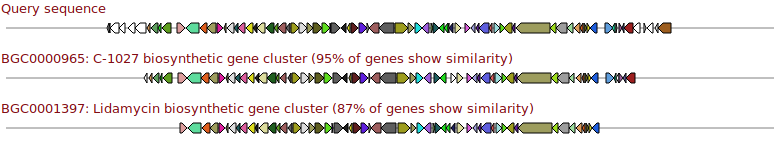
\includegraphics[width=1\linewidth]{contig4_cluster_search}
            \caption{Cluster search results for the identified cluster.}
            \label{fig:sub1}
        \end{subfigure}

        \begin{subfigure}[b]{\textwidth}
            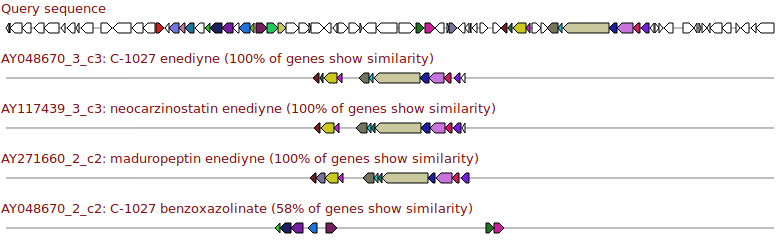
\includegraphics[width=1\linewidth]{contig4_subcluster_search}
            \caption{Subcluster search results for the identified cluster.}
            \label{fig:sub2}
        \end{subfigure}

        \caption[Cluster and subcluster search results for the cluster located on contig 4.]{\textbf{Cluster and subcluster search results for the cluster located on contig 4.} The 160~kb contig was submitted to AntiSMASH with the ClusterFinder option. Only the search results with the highest similarities are shown.}
        \label{fig:cluster_search}
    \end{figure}

% section genomic_analysis (end)
